\begin{Figure}
    
    \SECTION{2.4 Robustness of Chemical Switches}

    \TEXT{\bf Does parameter robustness imply noise robustness?}

   \begin{tikzpicture}
        \node [] (model) {
            \includegraphics[width=0.3\textwidth]{./images/model.png}
        };
    \end{tikzpicture} %
    \begin{tikzpicture}
        \node [] (timeline) {
            \includegraphics[width=0.6\textwidth]{./images/timeline.png}
        };
    \end{tikzpicture}

    \begin{tikzpicture}
        \node [] (timeseries) {
            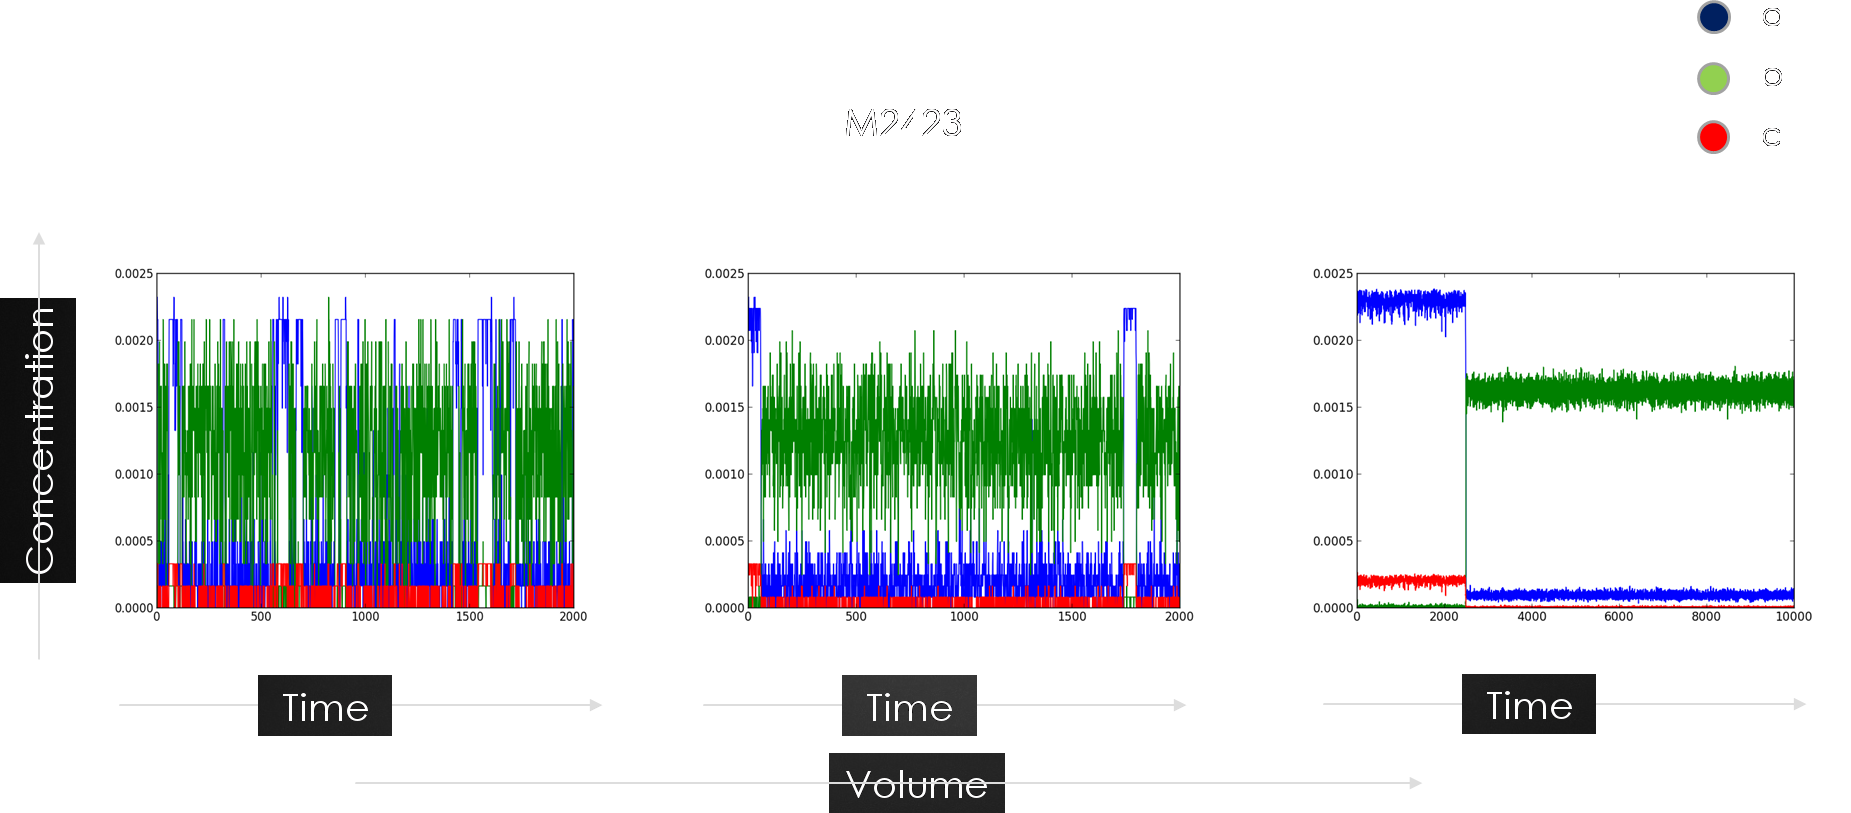
\includegraphics[trim=0 0 0 3cm,width=\textwidth,clip]{./images/TimeSeries.png}
        };
        \node [] (caption) at ([xshift=-4cm,yshift=0cm]timeseries.north) {
            \CAPTION{Stochastic simulation of bistable chemical models
                \hspace{1cm}}
        };

        \node[inner sep=1mm, minimum size=1.5cm,fill=blue,circle] (a) at
        (caption.east) {\Huge \textcolor{white}{a}};
        \node[inner sep=1mm, minimum size=1.5cm,fill=green,circle] (b) at
            ([xshift=2cm]a.east)  {\Huge b};
        \node[inner sep=1mm, minimum size=1.5cm,fill=red,circle] (c) at
        ([xshift=2cm]b.east) {\Huge c};

    \end{tikzpicture}

    \begin{tikzpicture}
        \node [] (density) {
            \includegraphics[width=0.5\textwidth]{./images/sahil_density.png}
        };
    \end{tikzpicture}
    \begin{tikzpicture}
        \node[] (ktseries) {
            \includegraphics[width=0.5\textwidth]{./images/KT_statistic_crop.png}
        };
    \end{tikzpicture}

    \vspace{1cm}
   \SECTION{2.5 GUI for Chemical and Electrical Models}

        \begin{tikzpicture}[ image/.style={xslant=0.5, yslant=0.0} ]
            \node []  {
                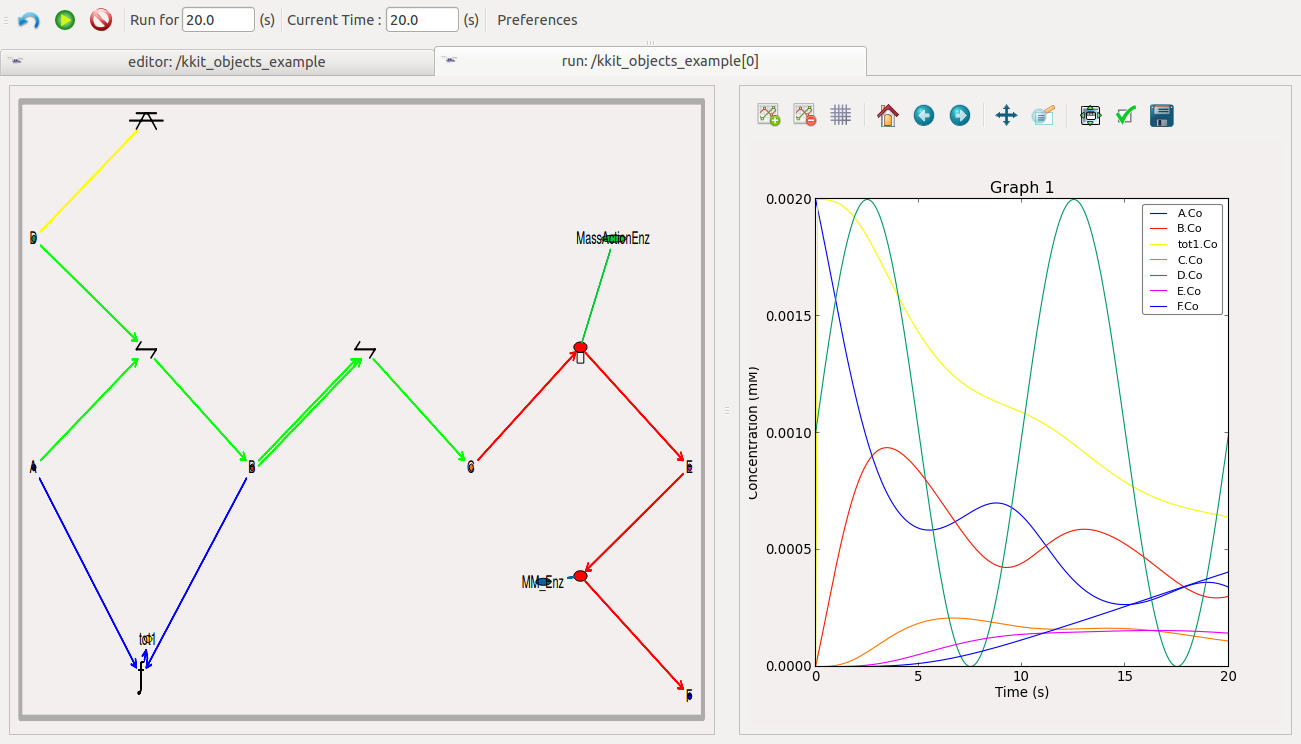
\includegraphics[width=0.5\textwidth]{./images/poster_runView.png}
            };
        \end{tikzpicture}%
        \begin{tikzpicture}
            \node [] (harsha) {
                \includegraphics[width=0.5\textwidth]{./images/moose_interface_electrical.png}
            };
        \end{tikzpicture}


    \vspace{1cm}
    \HEADING{3. Summary}

    \raggedright

    \TEXT{\bf We use models to:}
    \begin{itemize}

        \item \TEXT{Integrate many scales of neuronal data with basic
            physical/chemical principles.}
        \item \TEXT{Explain phenomena of plasticity, activity and neuronal
                coding.}
        \item \TEXT{Predict circuit mechanisms, plasticity rules, and emergent
            phenomena such as {decorrelation}, {robustness}, and
            {memory decay}.}

    \end{itemize}

 
\end{Figure}


